\documentclass[twocolumn]{article}

\usepackage{geometry}
\geometry{textwidth = 18cm,textheight = 24cm}

\usepackage{cite}
\usepackage{caption}
\usepackage{graphicx}
\usepackage{amsmath}
\usepackage{amssymb}
\usepackage{textcomp}
\usepackage{lmodern}
\usepackage{authblk}
  
\title{Fluxonic processing of photonic synapse events}
\author[1]{Jeffrey M. Shainline}
%\author[2]{someone else}
\affil[1]{National Institute of Standards and Technology, Boulder, CO, 80305}
%\affil[2]{somewhere else}
\date{\today}
\setcounter{Maxaffil}{0}
\renewcommand\Affilfont{\itshape\small}

\begin{document}

\twocolumn[
  \begin{@twocolumnfalse}
    \maketitle
    \begin{abstract}
    Much of the information processing performed by a neuron occurs in the dendritic arbor. For neural systems using light for communication, it is advantageous to convert to the electronic domain at synaptic terminals so dendritic computation can be performed with electrical circuits. Here we present circuits based on jjs and mis that act as dendrites processing signals from synapses receiving single-photon communication events with superconducting detectors. We show simulations of circuits performing basic logical operations such as AND and OR, which become correlation detectors when time dependence is added. These two-input logical operations straightforwardly extend to multiple inputs, and such a dendrites performs an intermediate thresholding nonlinearity between the synapses and the cell body. We further show how the signal from a single-photon synapse event can fan out locally in the electronic domain by roughly a factor of ten to enable the dendrites of the receiving neuron to process in multiple different ways. Such a technique makes efficient use of photons and energy while providing access to significantly more information regarding an afferent spike train.
    \vspace{3em}
    \end{abstract}
  \end{@twocolumnfalse}
]

%\tableofcontents

\section{\label{sec:introduction}Introduction}
%role of synaptic and dendrtic computation for neuronal information processing
A neuron is a complex information processing device, integrating signals from thousands of inputs and producing pulses when those signals reach threshold. These pulses, referred to as neuronal firing events, consume the most energy of any operation in the network. The neurons receiving the pulses must extract as much information as possible from each pulse. Neurons accomplish this through processing occurring in synapses and dendrites. Because neural information is based on temporal sequences of pulses, the relevant processing involves applying various temporal filters to extract relevant data. For example, synapses perform temporal filtering of pulse trains to identify rising edges (high pass) and to identify pulse trains exceeding some duration or number of pulses (low pass) \cite{}. Dendrites receive and further process synaptic signals. The operations performed by dendrites include leaky integration \cite{}, identification of coincidences \cite{} and sequences \cite{haah2015} between synapses from different neurons, and intermediate nonlinear thresholding transfer functions between groups of synapses and the cell body \cite{}. Inhibitory neurons in the network can temporarily suppress the activity of a dendrite to dynamically isolate information of interest, thereby adapting the structural network into myriad functional networks.

%context of emerging hardware
For hardware to be efficient for neural information processing, these synaptic and dendritic operations must be efficiently manifest in the constituent devices. We have argued elsewhere that light is promising for communication in neural systems, and that utilization of superconducting single-photon detectors enables communication at the lowest possible light levels \cite{shbu2017}. Subsequent work introduced circuits transducing single-photon communication events to the electronic domain for subsequent information processing \cite{sh2018,sh2018_full}. References \cite{sh2018} and \cite{sh2018_full} discussed basic synaptic functionality, plasticity, neuronal integration, thresholding, and the production of light during a neuronal firing event. Here we extend that work to consider additional synaptic and dendritic computational functions thought to be important for neural information processing. We discuss three elemental circuits that can be used as building blocks to perform many neural operations. These operations include leaky integration and temporal filtering of afferent pulse trains, detection of coincidences between activities of input neurons, inhibition, and long-term memory retention of synaptic activity.

\begin{figure} 
    \centering{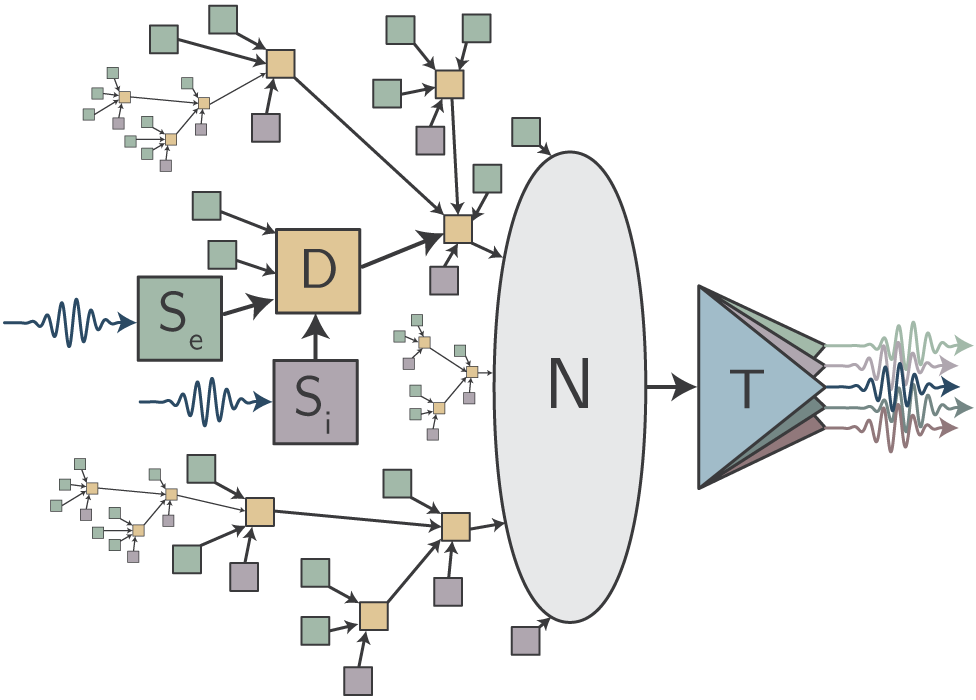
\includegraphics[width=8.6cm]{_01__schematic.png}}
	\captionof{figure}{\label{fig:schematic}Caption.}
\end{figure}
%summary of the model developed in this paper
Reference \cite{sh2018} considered a simple model of neuronal operation wherein synapses directly connect to neurons, and each neuron performs leaky integration of the synaptic activities with a single decay time constant, $\tau$. Within that model, each neuron is capable of answering the question, ``Is the integral of activity across all synapses in the last $\tau$ seconds greater than threshold?'' If the answer is yes, the neuron produces a pulse. While such a model may be useful for certain neuromorphic computations, it assumes that each neuron ignores or is incapable of utilizing nearly all the information to which it has access. The purpose of this paper is to consider a more elaborate model for neural information processing in which the dendritic arbor contains significantly more information about synaptic activities than a simple sliding sum. The model is illustrated schematically in Fig.\,\ref{fig:schematic}, which is intended to be an extension of a similar illustration used in Refs.\,\cite{sh2018} and \cite{sh2018_full}. We use the term, ``dendritic arbor'' to refer to a neuron's input synapses and dendrites collectively, and Fig.\,\ref{fig:schematic} is intended to illustrate the potential complexity of the dendritic arbor. In this work we develop circuits that will enable a neuron to answer subtle and varied questions, such as, ``How long has it been since neuron $i$ last produced a pulse?'' ``How many pulse trains have begun and then ceased on neuron $i$ in the last $\tau_i$ seconds?'' ``How many times have neurons $i$ and $j$ fired within $\tau_{ij}$ seconds of each other in the last $\tau_q$ seconds?''

\begin{figure} 
    \centering{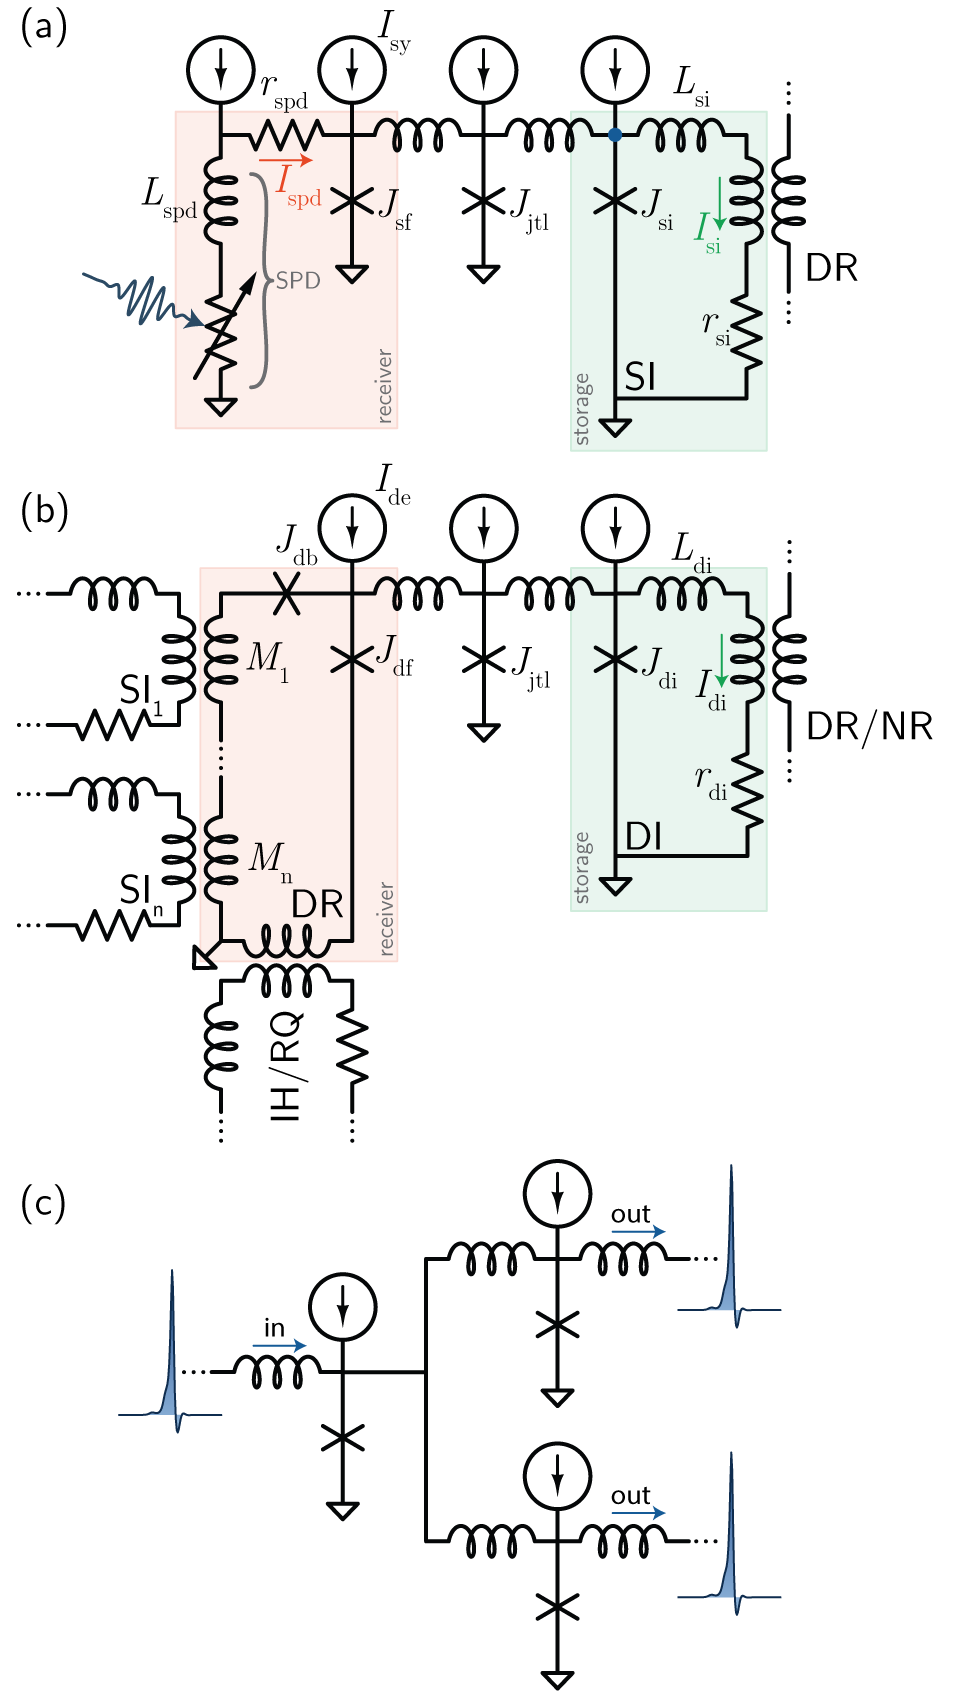
\includegraphics[width=8.6cm]{_02__circuits.png}}
	\captionof{figure}{\label{fig:circuits}Caption.}
\end{figure}
%specific contributions in this paper
In this work, we introduce circuits based on mutual inductors and Josephson junctions capable of providing the answers to these questions. This work is entirely theoretical and is based on time-domain circuit simulations of the three elemental circuits shown in Fig.\,\ref{fig:circuits} when arranged in various configurations. In Sec.\,\ref{sec:synapse} we review the basic operations of a synapse that transduces a single-photon communication event to the superconducting electronic domain for information processing, and in Sec.\,\ref{sec:short_term} we consider operations performed on pulse trains at a single synapse, usually associated with short-term plasticity and synaptic computation \cite{abre2004}. In Sec.\,\ref{sec:correlations} we consider the detection of coincidences between two or more synapses, and we show how the same circuits can be used with broken temporal symmetry to identify sequences of activity. In order for these various pieces of information to be utilized only when relevant, inhibition can be used to silence specific dendrites at appropriate times. Alternatively, it is possible to instead set a dendrite to silence by default, and provide access to its contents only at appropriate times. To accomplish this, we introduce a new type of dendritic readout that we refer to as rapid query, and we posit the utility of a dedicated class of rapid query neurons that, upon firing, ask question of sets of dendrites and cause those dendrites to report the answers to those questions up the dendritic tree toward the neuron cell body. Inhibition and rapid query are discussed in Sec.\,\ref{sec:inhibition_and_rapid_query}. 

%contributions continued
A central premise of the body of work represented by Refs.\,\cite{shbu2017,sh2018,sh2018_full,sh2018_ICRC} is that scalable neural systems will benefit from the fan-out and efficiency of few-photon communication. Yet when superconducting electronic circuits are employed for computation, these few-photon communication events dominate the energy budget. In Sec.\,\ref{sec:fluxonic_fanout} we discuss the use of superconducting splitters to make copies of photonic synapse events to that all of the questions discussed above can be answered by the dendritic arbor through processing of the signal from a single photon. Thus, the proposed hardware aspires to achieve greater than one-to-one-thousand fan-out in the photonic domain from each neuron to its thousands of connections. Subsequently, at each neuronal terminal, the hardware aspires to achieve an additional factor of roughly one-to-ten fan-out in the electronic domain, providing each receiving neuron with the capability of analyzing much more information about the synaptic activity. All fan-in occurs in the electronic domain as the dendritic arbor feeds its signals into the neuron cell body. Section \ref{sec:discussion} contains a discussion of the results.

\section{\label{sec:synapse}Photon-to-fluxon transduction at a synapse}
\begin{figure} 
    \centering{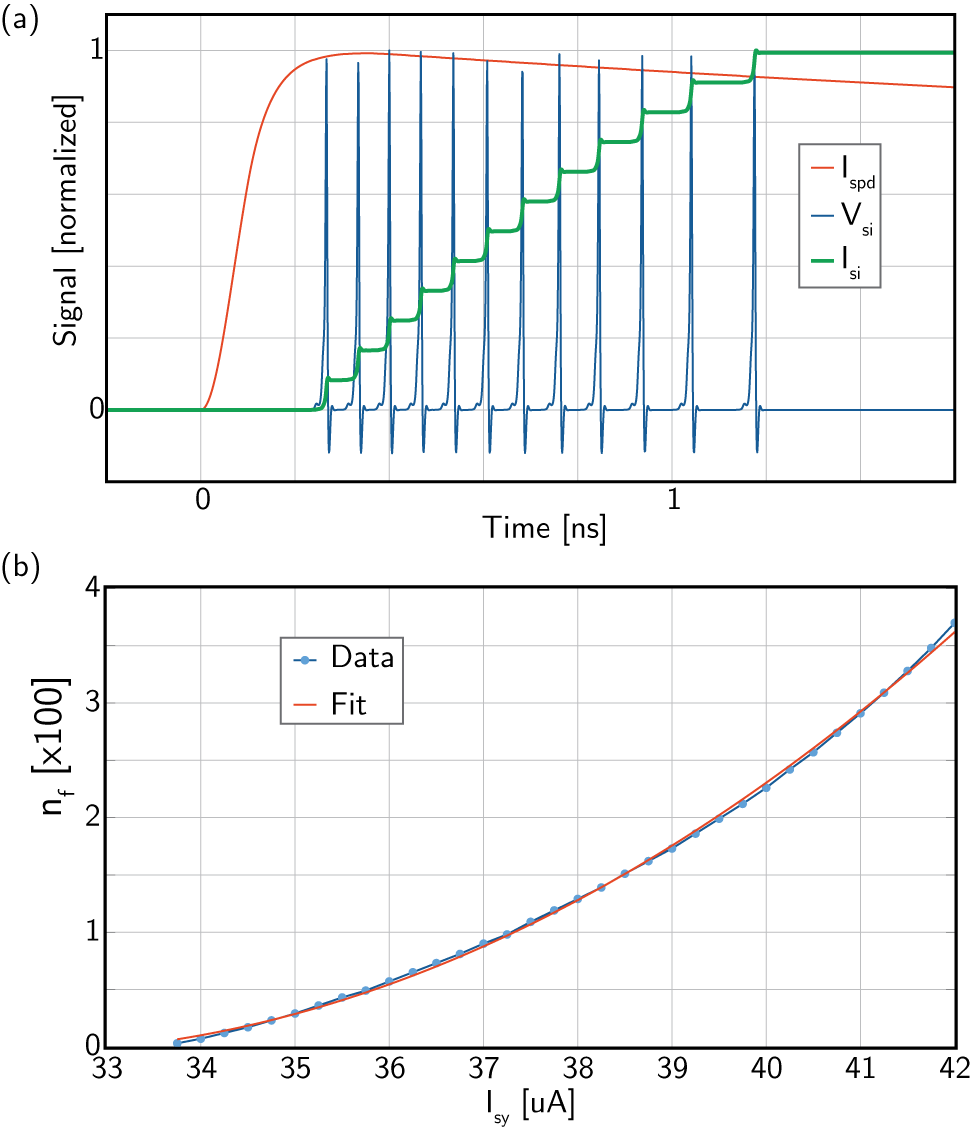
\includegraphics[width=8.6cm]{_03__sffg_basic.png}}
	\captionof{figure}{\label{fig:sffg_basic}Caption.}
\end{figure}
Analysis of fluxonic processing of photonic synapse events begins with consideration of the circuit that transduces a single-photon detection event to the superconducting electronic domain in the form of a series of fluxons. The circuit that accomplishes this is shown in Fig.\,\ref{fig:circuits}(a). This circuit was first introduced in Ref.\,\cite{sh2018} and described in more detail in Ref.\,\cite{sh2018_full}. The circuit comprises an initial receiver/transducer section, consisting of a superconducting-nanowire single-photon detector (SPD) \cite{gook2001,nata2012,liyo2013,mave2013} in parallel with a Josephson junction (JJ) \cite{ti1996,vatu1998,ka1999}. In the steady state, the SPD (drawn as a variable resistor in series with an inductor) has zero resistance, and thus its entire bias current flows directly through it to ground. The synaptic firing junction, $J_{\mathrm{sf}}$, is biased below its critical current ($I_{\mathrm{c}}$) by the synaptic bias current, $I_{\mathrm{sy}}$. Upon absorption of a photon, the variable resistor of the SPD switches temporarily to a high-resistance state ($\approx\,5$\,k$\Omega$) for a short duration ($\approx\,200$\,ps) \cite{yake2007}. The current through the SPD is diverted across a resistor ($I_{\mathrm{spd}}$ across $I_{\mathrm{spd}}$ in Fig.\,\ref{fig:circuits}(a)) and to $J_{\mathrm{sf}}$. At this point, the sum of the currents across $J_{\mathrm{sf}}$ exceeds $I_{\mathrm{c}}$, and the junction produces a series of fluxons \cite{ti1996,vatu1998,ka1999}. These fluxons propagate along the Josephson transmission line \cite{vatu1998,ka1999}, and are stored in the synaptic integration loop (SI). After the 200\,ps photon detection event, the bias current returns to the SPD with the time constant of $\tau_{\mathrm{spd}} = L_{\mathrm{spd}}/r_{\mathrm{spd}}$. This time constant has a minimum functional value determined by the electro-thermal properties of the nanowire \cite{yake2007}, and throughout this work we assume this time constant is fixed at $\tau_{\mathrm{si}} = 10$\,ns and the bias to the SPD is fixed at 10\,\textmu A. The number of fluxons created during a synaptic firing event depends on the net current across $J_{\mathrm{sf}}$ as well as the duration during which $J_{\mathrm{sf}}$ is biased above $I_{\mathrm{c}}$. With $\tau_{\mathrm{si}}$ and the bias to the SPD fixed, the number of fluxons, and thus the synaptic weight, are dynamically adaptable by changing the synaptic bias current, $I_{\mathrm{sy}}$. More details regarding $I_{\mathrm{sy}}$ and the associated plasticity mechanisms are given in Ref.\,\cite{sh2018_full}. 

The temporal activity of the circuit of Fig.\,\ref{fig:circuits}(a) during a synaptic firing event is shown in Fig.\,\ref{fig:sffg_basic}(a). Throughout this work, WRSpice \cite{wh1991} has been used to simulate all circuits, and all simulation parameters are given in the appendix. All JJs have $I_{\mathrm{c}} = 40$\,\textmu A and $\beta_{\mathrm{c}} = 0.95$. The red trace in Fig.\,\ref{fig:sffg_basic}(a) shows the current diverted from the SPD after a photon has been received. The blue trace shows the voltage pulses as the fluxons enter the SI loop. As each fluxon enters the loop, it introduces a discrete, fixed value of current given by $I_{\phi} = \Phi_0/L_{\mathrm{si}}$, where $\Phi_0 \approx 2\times10^{-15}$\,Wb is the magnetic flux quantum, and is $L_{\mathrm{si}}$ is the inductance of the synaptic integration loop. Throughout this work, we assume the value of $L_{\mathrm{si}}$ is chosen in design independently for each synapse and set in hardware at the time of fabrication. The green trace in Fig.\,\ref{fig:sffg_basic}(a) shows the increase in current as the fluxons enter the SI loop during a synaptic firing event. The discrete steps with each fluxon are evident, and the total amount of current added to the SI loop during a synaptic firing event depends on both the number of fluxons generated during the firing event (controlled dynamically by $I_{\mathrm{sy}}$) and the inductance of the SI loop (set in hardware as $L_{\mathrm{si}}$). 

The role of $I_{\mathrm{sy}}$ is to adapt the synaptic weight by changing the number of fluxons generated during a synaptic firing event. In Fig.\,\ref{fig:sffg_basic}(b) we show the number of fluxons generated during a synaptic firing event as a function of $I_{\mathrm{sy}}$. The fit shows close agreement with a second-order polynomial. This means of changing the synaptic weight has several important properties. First, it is slowly varying, so small changes in $I_{\mathrm{sy}}$ result in small changes in the synaptic efficacy. Second, the function is monotonic, so increases in $I_{\mathrm{sy}}$ always result in increased synaptic efficacy, while decreases in $I_{\mathrm{sy}}$ always result in decreases in synaptic efficacy. This is necessary to enable activity-based plasticity mechanisms \cite{somi2000,mage2012}, which have been explored in the context of these circuits in Ref.\,\ref{sh2018_full}. Third, the bias $I_{\mathrm{sy}}$ can be bounded so synaptic strength never exceeds a certain limit, and runaway activity is not possible. Finally, the integer number of fluxons generated can be made to cover a broad range so that analog synapses of relatively high bit depth can be achieved. Figure \ref{fig:sffg_basic}(b) shows that over eight bits (256 levels) can be utilized, and throughout this work we find the range of eight to 10 bits to be a comfortable working range for the circuits under consideration. This is, or course, much lower than the 64-bit processors used for high-arithmetic-depth numerical calculations. Yet neural computation benefits from performing lower-resolution operations with high efficiency with accuracy gained through redundancy and parallelism. 

\begin{figure} 
    \centering{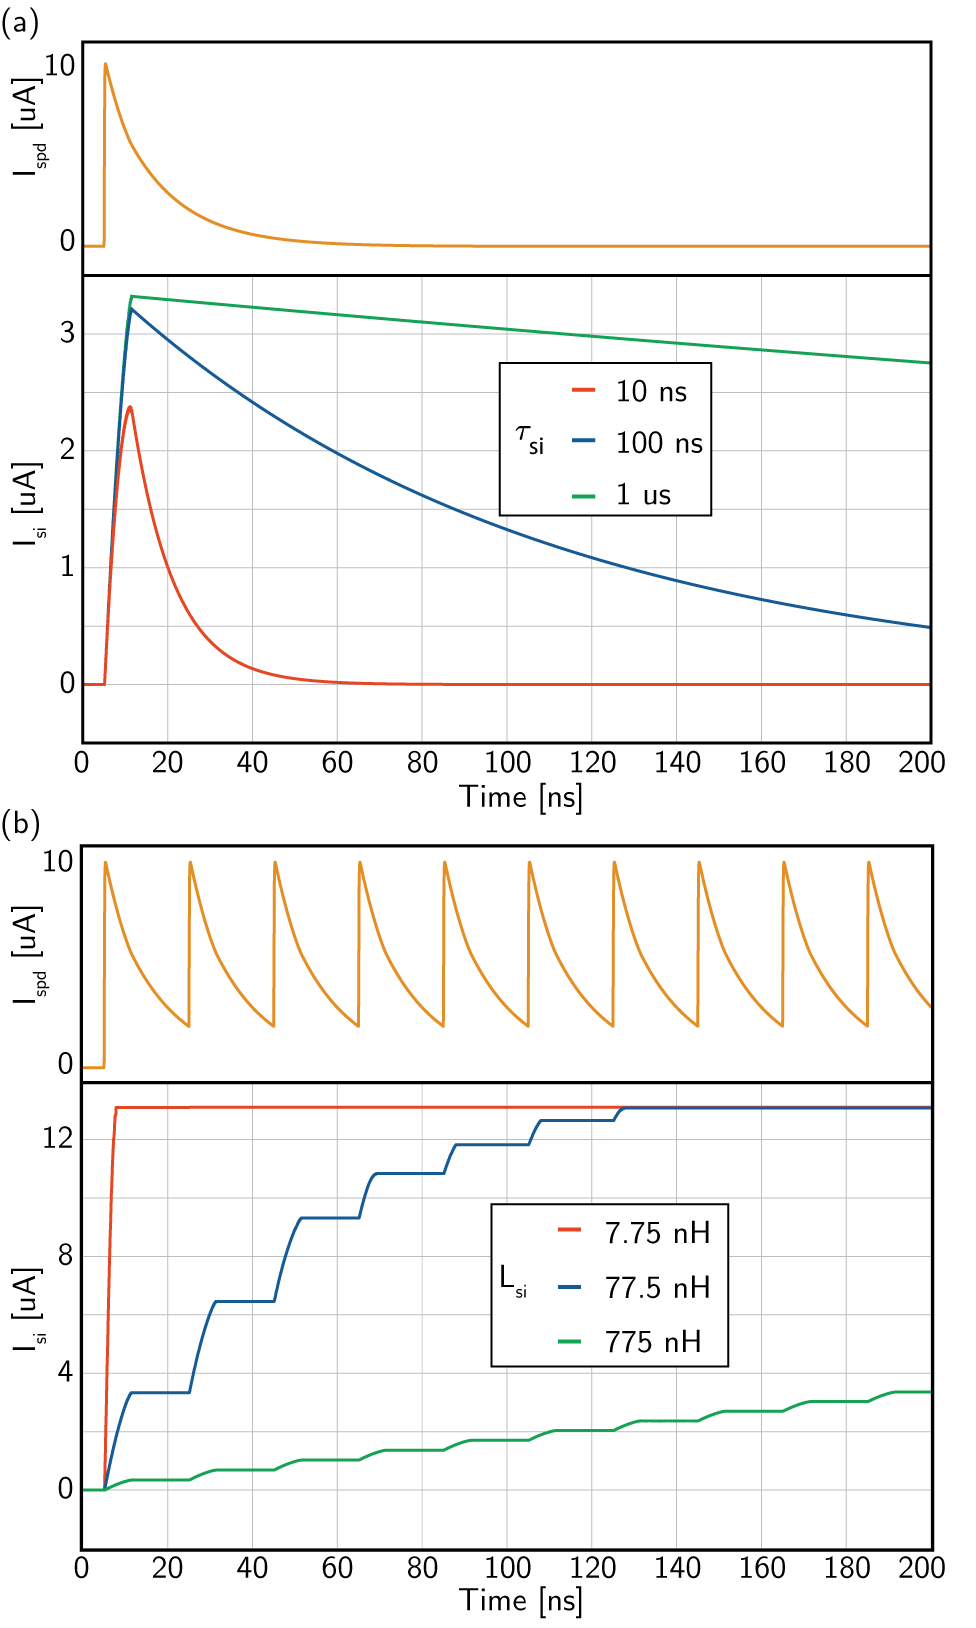
\includegraphics[width=8.6cm]{_04__sffg_betaL_tauSi.png}}
	\captionof{figure}{\label{fig:sffg_betaL_tauSi}Caption.}
\end{figure}
After a photonic communication event has been detected, the synaptic weight has been set as the number of fluxons created, and current has been added to the SI loop, further processing ensues. To start, the electrical current generated by the syanpse event can be stored for a chosen amount of time. This is determined by the leak rate of the SI loop, chosen in design and set in hardware by the time constant $\tau_{\mathrm{si}} = L_{\mathrm{si}}/r_{\mathrm{si}}$. Note that $\tau_{\mathrm{si}}$ is entirely independent of $\tau_{\mathrm{spd}}$, and because we consider superconducting circuits a memory of a synaptic event can persist indefinitely. Also note that while  the amount of current added to the SI loop during a synaptic firing event depends on $L_{\mathrm{si}}$, $r_{\mathrm{si}}$ can be chosen independently from $L_{\mathrm{si}}$, thereby enabling the amount of current and its storage time to separately selected. In Fig.\,\ref{fig:sffg_betaL_tauSi}(a) we show the temporal decay of current in the SI loop following a single synaptic firing event. The current can be released quickly, on the order of the SPD reset time of 10\,ns, or it can be stored 10 or 100 times longer to retain a memory of the event for as long as required. Here we show decay times spanning two orders of magnitude\textemdash from 10\,ns to 1\,\textmu s\textemdash, and it is likely that synaptic event retention times longer than this will not be necessary, as longer-term information storage is accomplished by modifying the plastic synaptic weight. 

%move this paragraph above previous paragraph
In biological neural systems, processing among local clusters of neurons occurs primarily through fast activity in the range of gamma frequencies (30\,Hz - 80\,Hz \cite{budr2004,bu2006}). This frequency range emerges because it reaches the upper limit of speed for the excitatory pyramidal neurons participating in the activity. In the superconducting optoelectronic hardware under consideration, this upper speed limit is near 100\,MHz, limited by the 10\,ns reset time of the SPDs in the synapses and of the transmitter circuits that generate neuronal firing events \cite{sh2018_full}. Therefore, we expect the neurons under consideration to demonstrate behavior similar to gamma oscillations, bursting with inter-spike intervals on the order of 10\,ns. Similarly, biological neural systems process information across the network as a whole through slower activity at theta frequencies of 4\,Hz - 8\,Hz \cite{budr2004,bu2006}. Naively mapping this scaling onto the system under consideration, we pay particular attention to gamma oscillations occurring at 100\,MHz as well as theta oscillations occurring at 10\,MHz. It is for this reason that we have considered the values of $\tau_{\mathrm{si}}$ in Fig.\,\ref{fig:sffg_betaL_tauSi}(a), and based on these consideration we must also consider the behavior of a synapse in response to a spike train corresponding to spike trains at gamma frequencies. 

In Fig.\,\ref{fig:sffg_betaL_tauSi}(b) we show the integrated current in an SI loop as a function of time in response to a periodic train of pulses with 10\,ns inter-spike interval. Here we fix $\tau_{\mathrm{si}} = \infty$ and vary the inductance of the loop, $L_{\mathrm{si}}$, which changes amount of current added to the loop with each fluxon and therefore each synaptic firing event. In these simulations, the value of $I_{\mathrm{sy}}$ was fixed at 38\,\textmu A, so 129 flux quanta are generated during the synaptic firing event. With a small value of $L_{\mathrm{si}}$, the quantity $I_{\phi} = \Phi_0/L_{\mathrm{si}}$ is large, and the loop saturates after a single synaptic firing event. With an intermediate value of $L_{\mathrm{si}} = 77.5$\,nH, seven synaptic firing events fill the loop, and with a large value of $L_{\mathrm{si}} = 775$\,nH, the loop can hold the activity from nearly 100 synaptic firing events with this value of $I_{\mathrm{sy}}$. This saturation occurs because each fluxon entering the loop induces a current countering the bias to the JJ. After some number of fluxons have been added, the additional bias current resulting from the synaptic firing event is no longer sufficient to raise $J_{\mathrm{si}}$ above $I_{\mathrm{c}}$. 

In general, the storage capacity of a superconducting loop with a JJ is characterized by the parameter $\beta_{\mathrm{L}} = 2\pi L I_c/\Phi_0$, and $\beta_{\mathrm{L}}$ quantifies the number of fluxons that can be stored. 

\begin{figure} 
    \centering{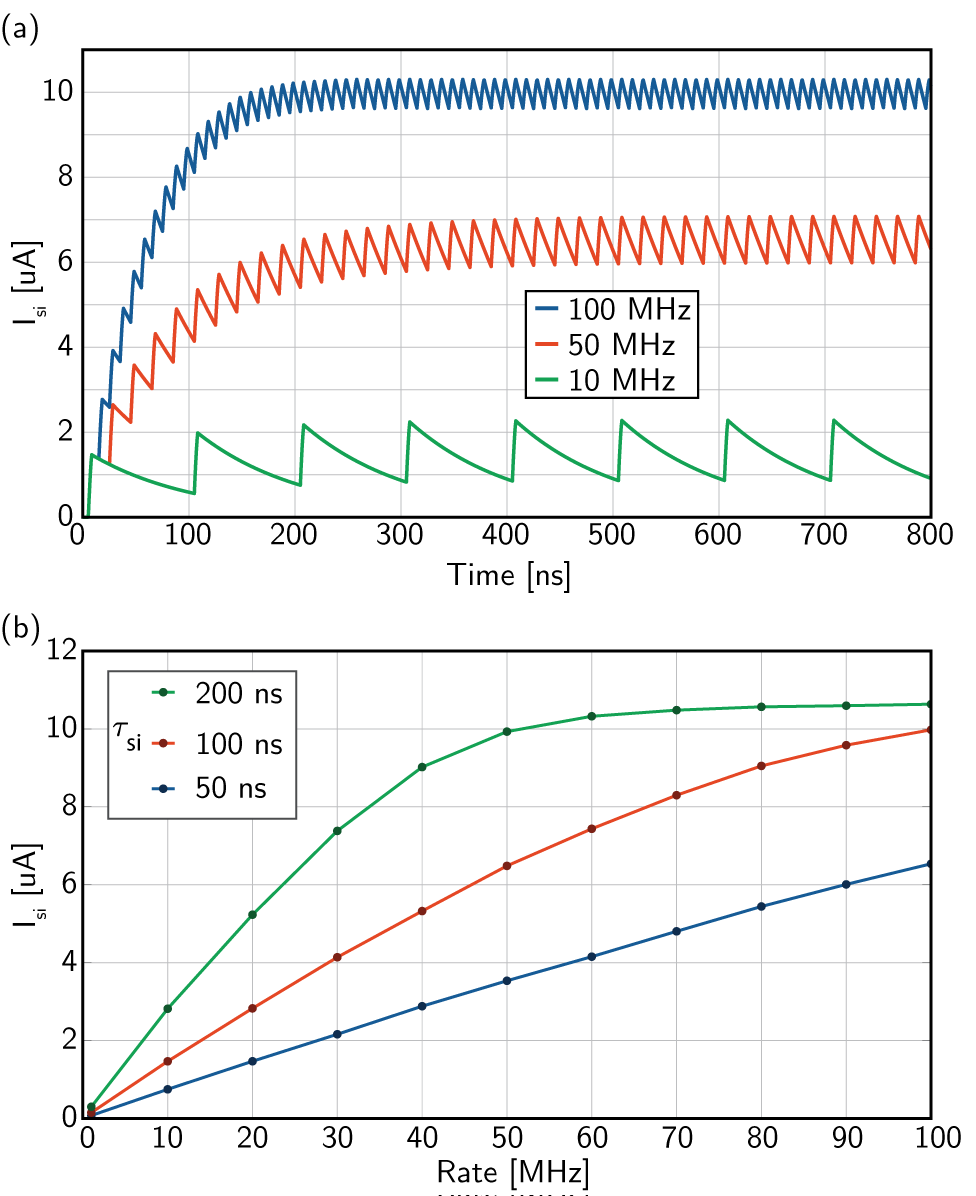
\includegraphics[width=8.6cm]{_05__sffg_rate_conversion.png}}
	\captionof{figure}{\label{fig:sffg_rate_conversion}Caption.}
\end{figure}

\section{\label{sec:short_term}Operations on pulse trains at a single synapse}

\begin{figure} 
    \centering{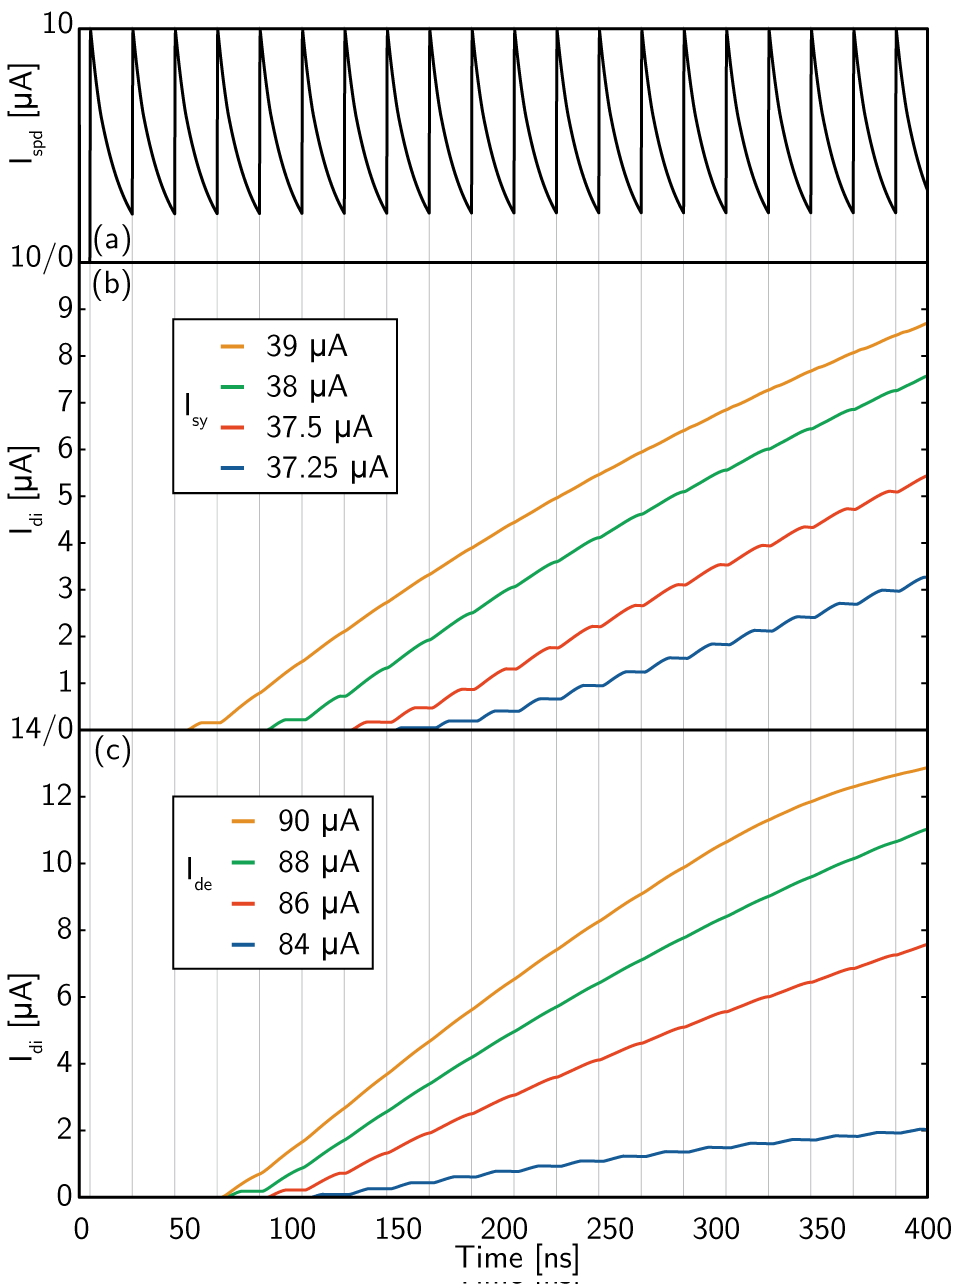
\includegraphics[width=8.6cm]{_06__si_di_facilitating.png}}
	\captionof{figure}{\label{fig:si_di_facilitating}Caption.}
\end{figure}

\begin{figure} 
    \centering{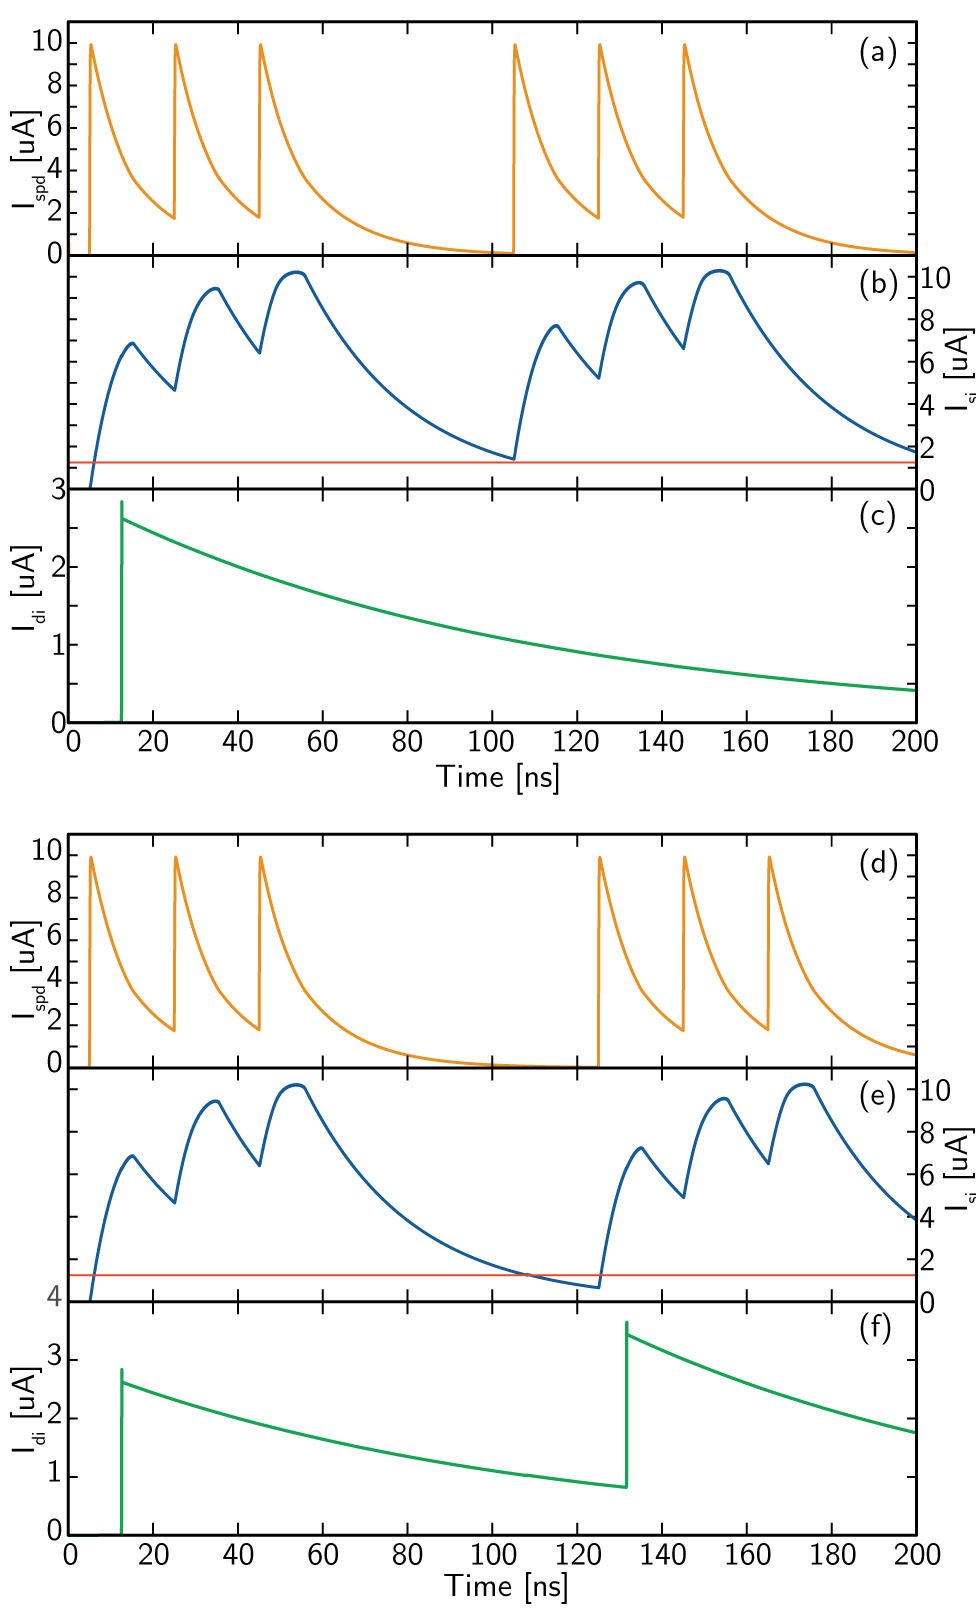
\includegraphics[width=8.6cm]{_07__si_dcsfq_depressing.png}}
	\captionof{figure}{\label{fig:si_dcsfq_depressing}Caption.}
\end{figure}

\section{\label{sec:correlations}Detecting correlations between neurons}

\begin{figure} 
    \centering{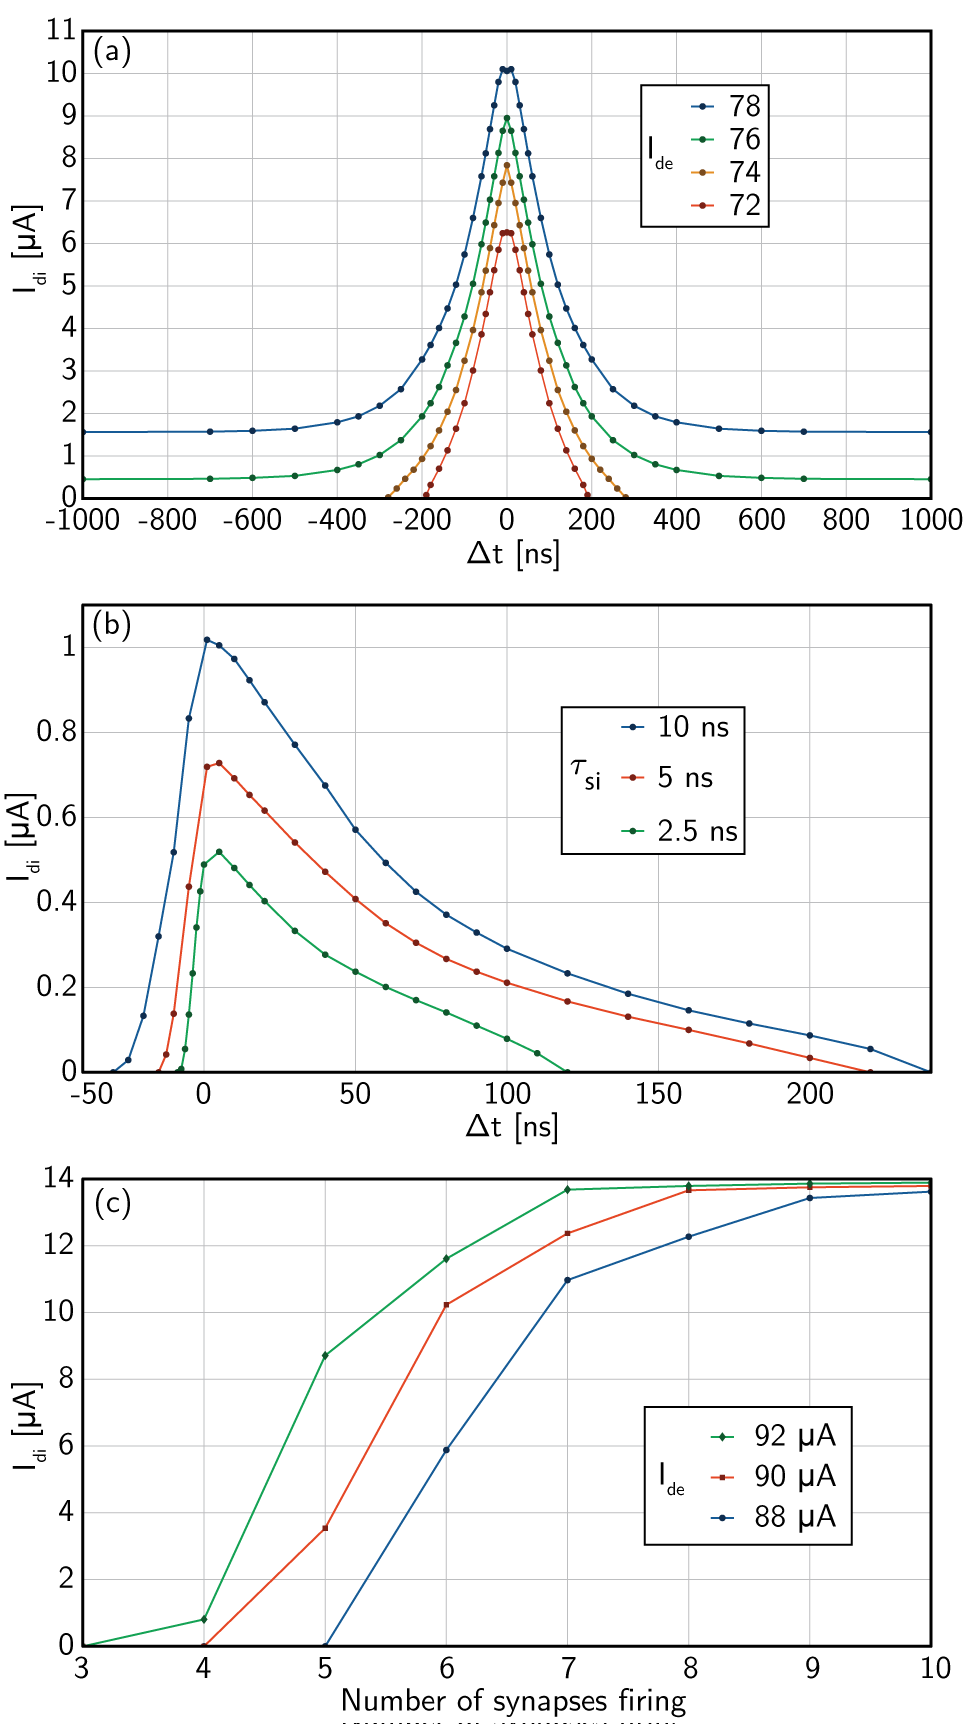
\includegraphics[width=8.6cm]{_08__poly_si_di.png}}
	\captionof{figure}{\label{fig:poly_si}Caption.}
\end{figure}

\section{\label{sec:inhibition_and_rapid_query}Inhibition and rapid query}

\begin{figure} 
    \centering{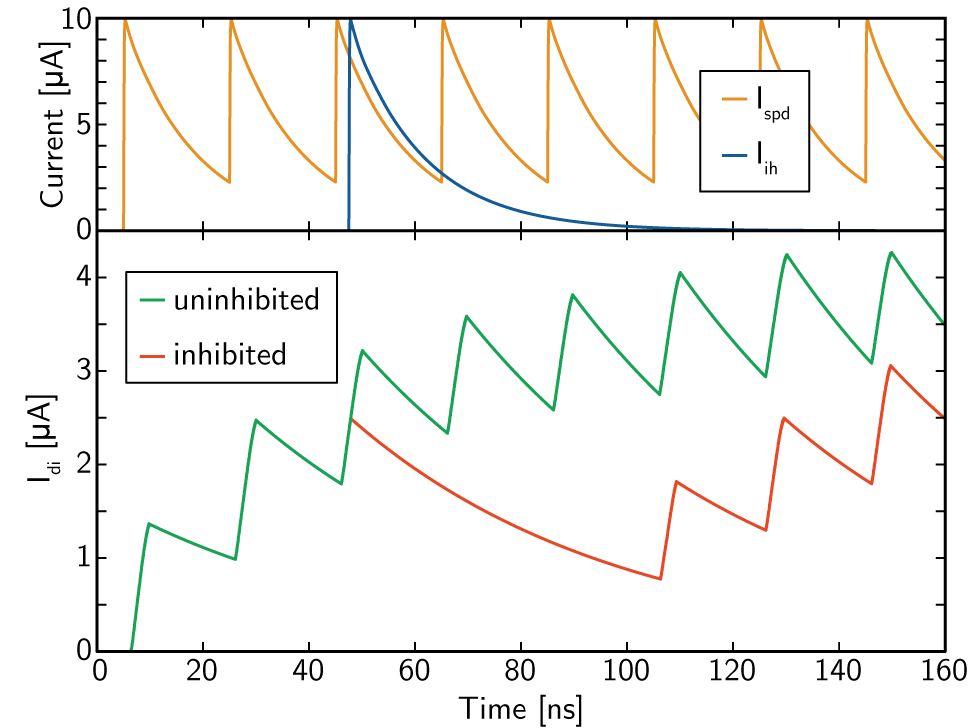
\includegraphics[width=8.6cm]{_09__si_di_inhibition.png}}
	\captionof{figure}{\label{fig:si_di_inhibition}Caption.}
\end{figure}

\begin{figure} 
    \centering{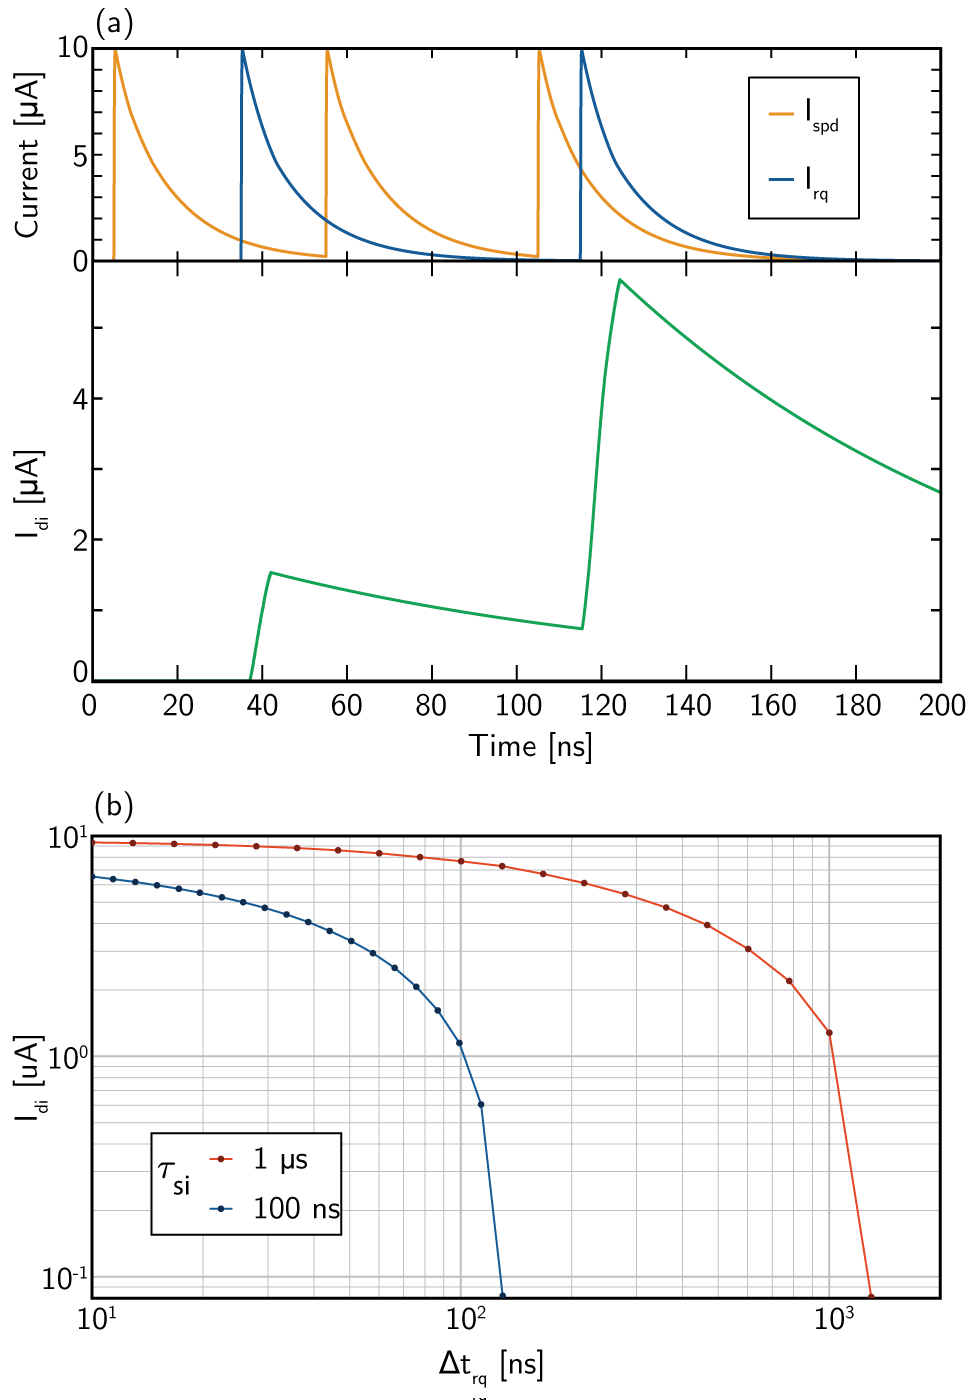
\includegraphics[width=8.6cm]{_10__si_di_rapid_query.png}}
	\captionof{figure}{\label{fig:si_di_rapid_query}Caption.}
\end{figure}

To our knowledge, there is no analog of a rapid query neuron in the biological domain, yet we 

\section{\label{sec:fluxonic_fanout}Fanout to multiple synapses from the same neuron}

\begin{figure} 
    \centering{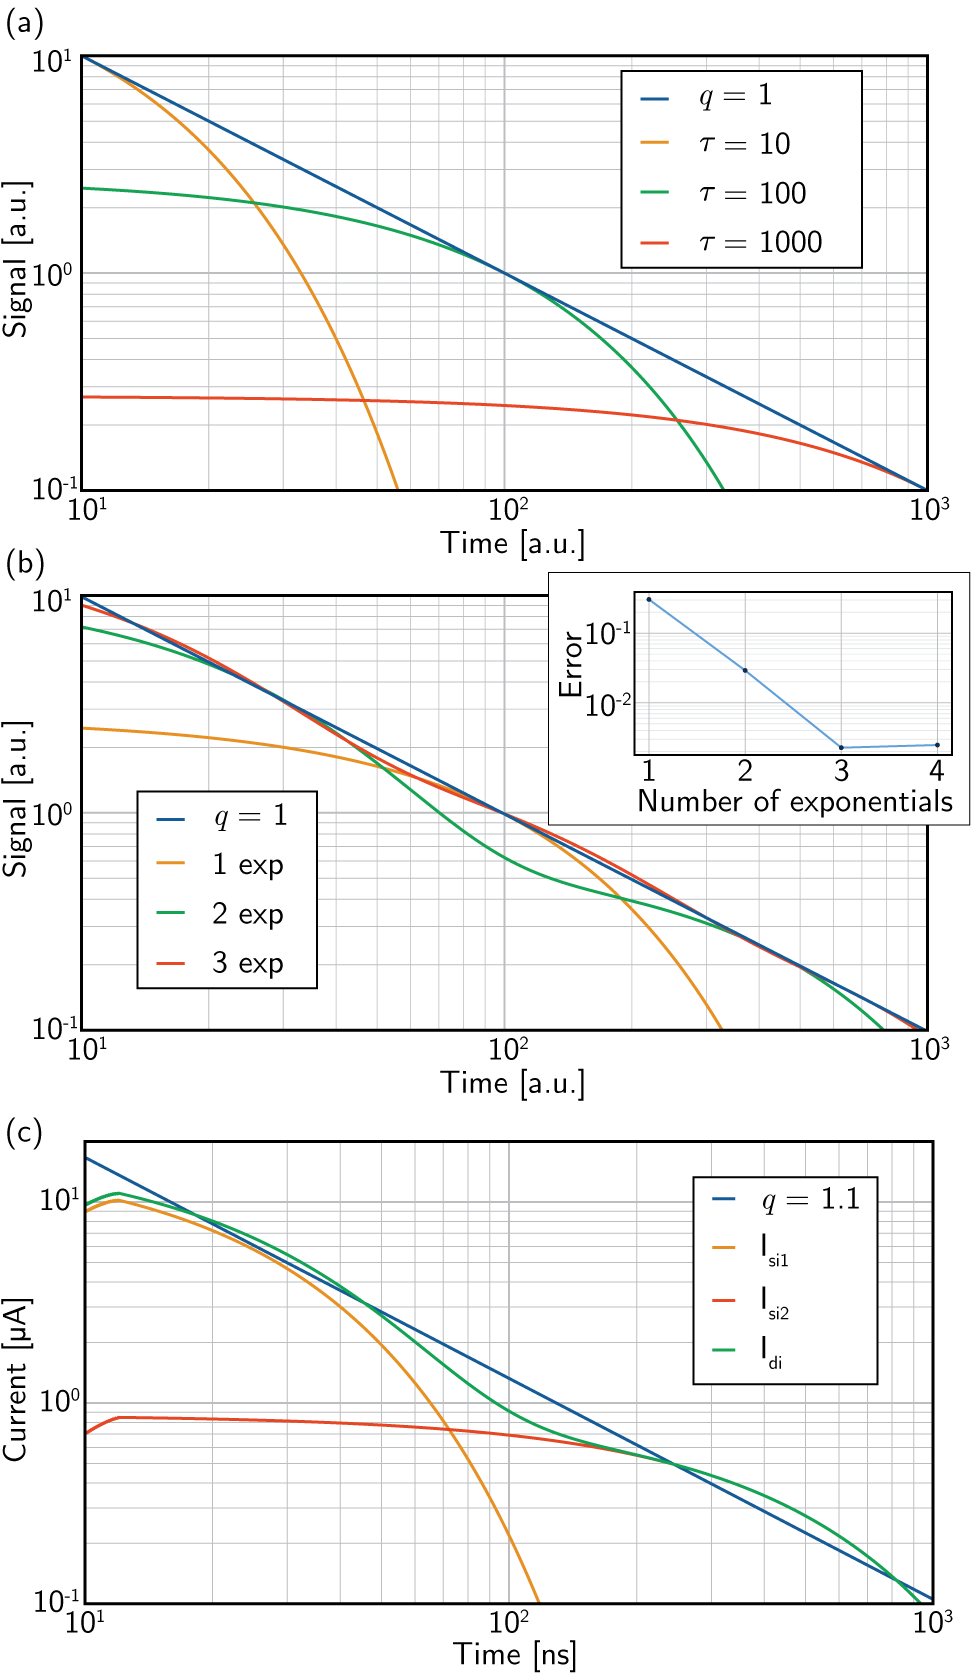
\includegraphics[width=8.6cm]{_11__power_law_time_decay.png}}
	\captionof{figure}{\label{fig:power_law_time_decay}Caption.}
\end{figure}

\section{\label{sec:discussion}Discussion}
	
\newpage
\appendix

\bibliographystyle{unsrt}
\bibliography{fluxonic_processing_of_photonic_synapse_events}

\end{document}